\documentclass[]{beamer}
\mode<presentation>
% Time-stamp: <2016-06-14 10:20:06 (jmiller)>

% beamer stuff
% Gives us the bottom line with all the goodies
\useoutertheme{infolines}
% Just the theme to use. Should be built into bemaer. Setting the
% height gets rid of a whole lot of whitespace
\usetheme[height=7mm]{Rochester}
\usefonttheme{serif}
% Usually beamer gives you navigation hyperlinks on the bottom
% right. I turned this off. It's annoying.
\setbeamertemplate{navigation symbols}{} 
% Makes my text boxes look pretty
\setbeamertemplate{blocks}[rounded][shadow=true] 
% Makes my bullet points 3d balls
\setbeamertemplate{items}[ball]

% Josh's packages
\usepackage{multimedia}
\usepackage{tabularx}
\usepackage{booktabs}
\usepackage{subfigure}
\usepackage{graphicx}
\usepackage{amsmath}
\usepackage{latexsym}
\usepackage{mathrsfs}

% Packages for me
\usepackage{amsmath,amssymb,latexsym}
\usepackage[mathscr]{eucal}
\usepackage{mathrsfs}
\usepackage{verbatim}
\usepackage{braket}
\usepackage{listings}
\usepackage{amsthm}
\usepackage{xcolor}
%\usepackage[usenames,dvipsnames,svgnames,table]{xcolor}
\usepackage{fancybox}
\usepackage{animate}
% \usepackage{media9}
\usepackage{multicol}
\usepackage{mdframed}
%\usepackage{scalerel}
\usepackage{hyperref}

% Macros

%Blackboard Bold
\newcommand{\R}{\mathbb{R}}
\newcommand{\Z}{\mathbb{Z}}
\newcommand{\N}{\mathbb{N}}
\newcommand{\Q}{\mathbb{Q}}
\newcommand{\A}{\mathbb{A}}
\newcommand{\E}{\mathbb{E}}
% other
\newcommand{\eval}{\biggr\rvert} %evaluated at
\newcommand{\myvec}[1]{\mathbf{#1}} % vectors for me
% total derivatives 
\newcommand{\diff}[2]{\frac{d #1}{d #2}} 
\newcommand{\dd}[1]{\frac{d}{d #1}}
% partial derivatives
\newcommand{\pd}[2]{\frac{\partial #1}{\partial #2}} 
\newcommand{\pdd}[1]{\frac{\partial}{\partial #1}} 
% Order operator
\DeclareRobustCommand{\orderof}{\ensuremath{\mathcal{O}}}

% tikz
\usepackage{tikz}
\usetikzlibrary{arrows}
\usepackage{pgfplots}


% Keys to support piece-wise uncovering of elements in TikZ pictures:
% \node[visible on=<2->](foo){Foo}
% \node[visible on=<{2,4}>](bar){Bar}   % put braces around comma expressions
% 
% Internally works by setting opacity=0 when invisible, which has the 
% adavantage (compared to \node<2->(foo){Foo} that the node is always there, hence
% always consumes space plus that coordinate (foo) is always available.
% 
% The actual command that implements the invisibility can be overriden
% by altering the style invisible. For instance \tikzsset{invisible/.style={opacity=0.2}}
% would dim the "invisible" parts. Alternatively, the color might be set to white, if the
% output driver does not support transparencies (e.g., PS) 
% 
\tikzset{
  invisible/.style={opacity=0},
  visible on/.style={alt={#1{}{invisible}}},
  alt/.code args={<#1>#2#3}{%
    \alt<#1>{\pgfkeysalso{#2}}{\pgfkeysalso{#3}} % \pgfkeysalso doesn't change the path
  },
}

% some nice flowchart features
\tikzset{
    mynode/.style={rectangle,rounded corners,draw=black, top color=white, bottom color=yellow!50,very thick, inner sep=1em, minimum size=3em, text centered},
    myarrow/.style={->, >=latex', shorten >=1pt, thick},
    mylabel/.style={text width=7em, text centered} 
}  

% define a really nice visible "purple"
\definecolor{gimppurple}{HTML}{AD26FB}
% a light grey
\definecolor{lightgrey}{HTML}{E0E0E0}
% for highlighting
\definecolor{deepblue}{rgb}{0,0,0.5}
\definecolor{deepred}{rgb}{0.6,0,0}
\definecolor{deepgreen}{rgb}{0,0.5,0}

% fonts
% Default fixed font does not support bold face
\DeclareFixedFont{\ttb}{T1}{txtt}{bx}{n}{10} % for bold
\DeclareFixedFont{\ttm}{T1}{txtt}{m}{n}{10}  % for normal

% Python style for highlighting
\newcommand\pythonstyle{\lstset{
language=Python,
basicstyle=\footnotesize\ttm,
otherkeywords={self},
keywordstyle=\ttb\color{deepblue},
emph={__init__},           
emphstyle=\ttb\color{deepred},
commentstyle=\ttfamily\color{deepred},
stringstyle=\color{deepgreen},
frame=tb,                     
showstringspaces=false        
}}

% Python environment
\lstnewenvironment{python}[1][]
{
\pythonstyle
\lstset{#1}
}
{}

\newcommand{\backupbegin}{
   \newcounter{finalframe}
   \setcounter{finalframe}{\value{framenumber}}
}
\newcommand{\backupend}{
   \setcounter{framenumber}{\value{finalframe}}
}

% a macro for a useful transition slide
\newcommand{\transitionslide}[1]{
  \begin{frame}[plain]
  \vfill
  \centering
  \begin{beamercolorbox}[sep=8pt,center,shadow=true,rounded=true]{title}
    \usebeamerfont{title}{#1}
  \end{beamercolorbox}
  \vfill
\end{frame}
}

\title[SIO \& yt]{SimulationIO and yt}
\author[J. Miller]{Jonah M. Miller}
\institute[PI]{\color{blue}Perimeter Institute for Theoretical Physics}

\date[ET Workshop]{\color{black}Einstein Toolkit Workshop\\Wednesday, June 15}

\begin{document}

\begin{frame}[plain]
\titlepage
\end{frame}

\begin{frame}
  \frametitle{What are they?}
  \begin{itemize}
  \item {\color{blue}\href{https://github.com/eschnett/SimulationIO}{SimulationIO}} is a library
    \begin{itemize}
    \item Written by Erik Schnetter
    \item Open source
    \item Meant to be a \textit{high-level} description of the output of
      potentially many simulations
    \item Abstracts away simulation details
    \item Describes an API
    \item Uses category theory to cleanly remove ambiguities
    \end{itemize}
  \item {\color{blue}\href{http://yt-project.org/}{yt}} is a
    visualization (and data analysis) toolkit
    \begin{itemize}
    \item Open source
    \item Community driven
    \item Written in Python
    \item Very hack-able
    \end{itemize}
  \end{itemize}
\end{frame}

\begin{frame}
  \frametitle{What do we care about in a simulation?}
  \begin{tikzpicture}
    \draw[ultra thick,->] (7,3) -- (4,1.5);
    \node[inner sep=0pt] at (2,2) {\includegraphics[width=4cm,trim={0cm 0cm 0cm 0cm},clip]{figures/surface-scatter-small}};
    \node[inner sep=0pt] at (9,3.5) {\includegraphics[width=8cm,trim={0cm 0cm 0cm 0cm},clip]{figures/surface-scatter}};
    \draw[ultra thick,->] (5,7) -- (7,4);
    \node[inner sep=0pt] at (4,6) {\includegraphics[width=8cm,trim={0.5cm 0cm 0cm 1.75cm},clip]{figures/surface-smooth}};
  \end{tikzpicture}
\end{frame}

\begin{frame}
  \frametitle{What do we care about in a simulation?}
  \begin{center}
    \includegraphics[width=12cm]{figures/wavey}
  \end{center}
\end{frame}

\begin{frame}
  \frametitle{What do we care about in a simulation?}
    \begin{center}
    \includegraphics[width=6cm]{figures/fourpatches.png}
    \includegraphics[width=6cm]{figures/sixpatches.png}
  \end{center}
  Schnetter \textit{et al} 2006 Class. \textit{Quantum Grav.} \textbf{23} S553\\
  Pollney \textit{et al} 2011 \textit{Phys. Rev. D} \textbf{83} 044045
\end{frame}

\begin{frame}
  \frametitle{Other efforts}
  \begin{columns}
    \column{6cm}
  \begin{itemize}
  \item {\color{blue}\href{http://vish.fiberbundle.net/documentation/the-fiber-bundle-data-model/}{Fiber Bundle}} by Werner Benger
  \item {\color{blue}\href{https://bitbucket.org/DrWhat/pycactuset}{PostCactus}} by Wolfgang Kastaun
  \item {\color{blue}\href{http://simulationtools.org/}{Simulation Tools}} by Ian Hinder and Barry Wardell
  \item {\color{blue}\href{https://bitbucket.org/dradice/scidata}{scidata}} by David Radice
  \item {\color{blue}\href{https://bitbucket.org/fguercilena/rugutils}{rugutils}} by Federico Guercilena
  \item {\color{blue}\href{https://bitbucket.org/knarrff/pycactus}{pycactus}} by Roberto De Pietri, Francesco Maione, and Frank L\"{o}ffler
  \end{itemize}
  \column{6cm}
  \begin{center}
    \includegraphics[width=6cm]{figures/simulation_tools_example.png}
  \end{center}
  \end{columns}
\end{frame}

\begin{frame}
  \frametitle{Projects as Directed Graphs}
  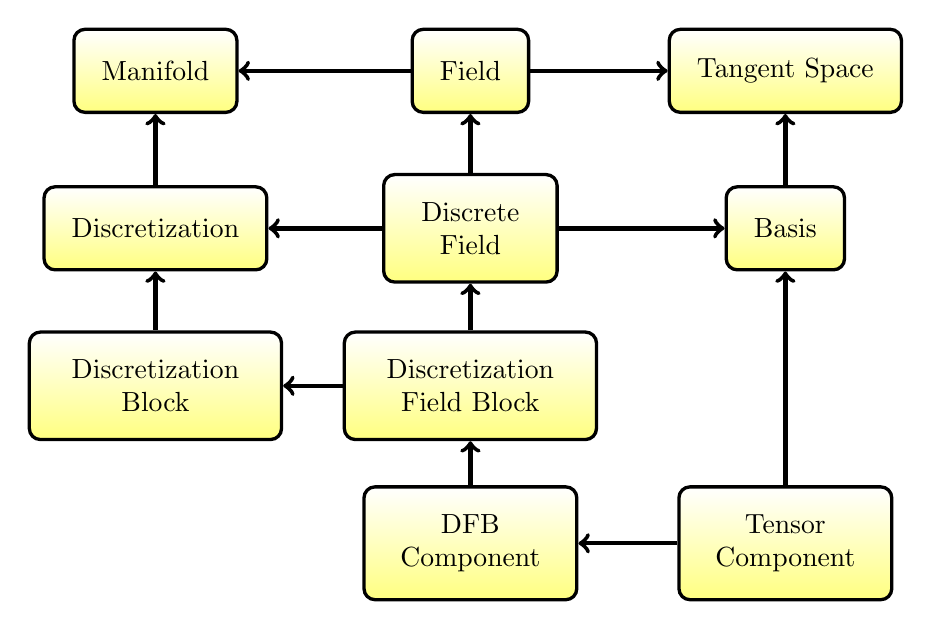
\begin{tikzpicture}
    \draw (1,8) node[mynode] (manifold) {Manifold};
    \draw (1,6) node[mynode] (discretization) {Discretization};
    \draw[ultra thick,<-] (manifold) -- (discretization);
    \draw (1,4) node[mynode,text width=2.5cm,align=center] (discb) {Discretization Block};
    \draw[ultra thick,<-] (discretization) -- (discb);
    \draw (5,8) node[mynode] (field) {Field};
    \draw[ultra thick,<-] (manifold) -- (field);
    \draw (5,6) node[mynode,text width=1.5cm,align=center] (discrete field) {Discrete Field};
    \draw[ultra thick,<-] (field) -- (discrete field);
    \draw[ultra thick,->] (discrete field) -- (discretization);
    \draw (5,4) node[mynode,text width=2.5cm,align=center] (dfb) {Discretization Field Block};
    \draw[ultra thick,->] (dfb) -- (discrete field);
    \draw[ultra thick,->] (dfb) -- (discb);
    \draw (5,2) node[mynode,text width=2.cm,align=center] (dfbc) {DFB Component};
    \draw[ultra thick,->] (dfbc) -- (dfb);
    \draw (9,8) node[mynode] (tangent) {Tangent Space};
    \draw[ultra thick,->] (field) -- (tangent);
    \draw (9,6) node[mynode] (basis) {Basis};
    \draw[ultra thick,<-] (tangent) -- (basis);
    \draw[ultra thick,->] (discrete field) -- (basis);
    \draw (9,2) node[mynode,text width=2.cm,align=center] (component) {Tensor Component};
    \draw[ultra thick,->] (component) -- (basis);
    \draw[ultra thick,->] (component) -- (dfbc);
  \end{tikzpicture}
\end{frame}

\begin{frame}
  \frametitle{AMR in SimulationIO}
  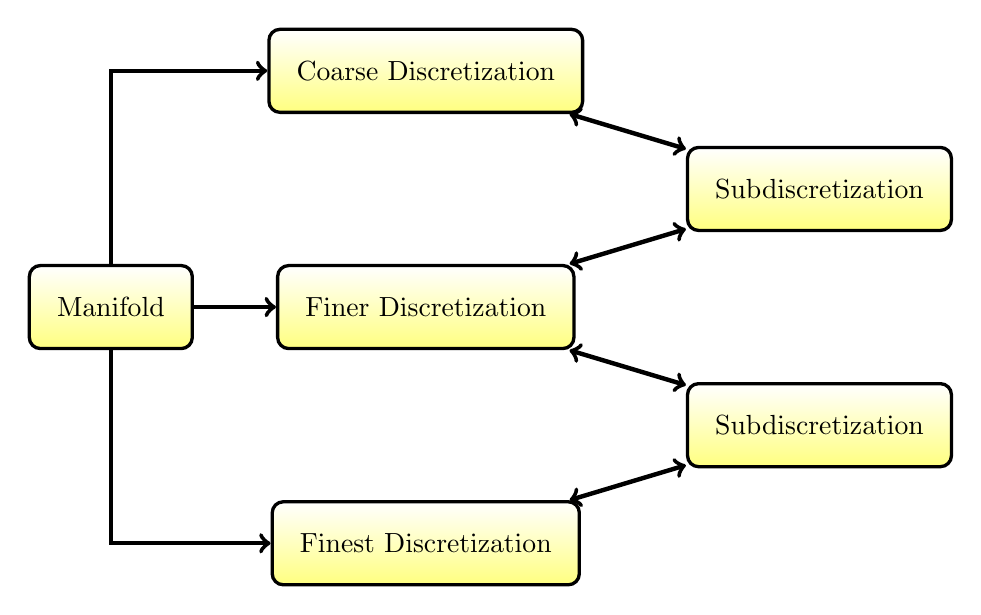
\begin{tikzpicture}
    \draw (0,5) node[mynode] (manifold) {Manifold};
    \draw (4,8) node[mynode] (rdiscretization) {Coarse Discretization};
    \draw (4,5) node[mynode] (discretization1) {Finer Discretization};
    \draw (4,2) node[mynode] (discretization2) {Finest Discretization};
    \draw (9,6.5) node[mynode] (subdiscretization1) {Subdiscretization};
    \draw (9,3.5) node[mynode] (subdiscretization2) {Subdiscretization};
    \draw[ultra thick,->] (manifold) -- (0,8) -- (rdiscretization);
    \draw[ultra thick,->] (manifold) -- (discretization1);
    \draw[ultra thick,->] (manifold) -- (0,2) -- (discretization2);
    \draw[ultra thick,<->] (rdiscretization) -- (subdiscretization1);
    \draw[ultra thick,<->] (subdiscretization1) -- (discretization1);
    \draw[ultra thick,<->] (discretization1) -- (subdiscretization2);
    \draw[ultra thick,<->] (subdiscretization2) -- (discretization2);
  \end{tikzpicture}
\end{frame}

\begin{frame}[fragile]
  \frametitle{SimulationIO Utilities}
  \begin{itemize}
  \item {\color{blue}\lstinline$sio-list$} is a utility for listing the contents of
    a file
\begin{lstlisting}[language=bash]
  sio-list file.s5
\end{lstlisting}
  \item {\color{blue}\lstinline$sio-convert-carpet-output$} converts a
    sequence of hdf5 files to an s5 file.
\begin{lstlisting}[language=bash]
  sio-convert-carpet-output out.s5 file_*.h5
\end{lstlisting}
  \end{itemize}
\end{frame}

\begin{frame}[fragile]
  \frametitle{SimulationIO Python API}
  \begin{python}
    import pysimulationio
    project,file_handle = SIO.readProject(filename)
    field = project.fields['rho']
    dcf = field.discretefields['rho']
    for dcfb in\
    dcf.discretefieldblocks.itervalues():
        for dcfbc in\
        dcfb.discretefieldblockcomponents:
            c = dcfbc.values()[0]
            dset = c.getData_DataSet()
            data = np.array(dset.read_double())
    file_handle.close()
  \end{python}
\end{frame}

\transitionslide{\Huge yt}

\begin{frame}
  \frametitle{volume rendering}
  \begin{center}
    \animategraphics[height=8cm,every=1,autoplay,loop]{6}{figures/psi4r-it-1024/psi4r-iteration-1024-volume-f-}{00}{32}
  \end{center}
\end{frame}

\begin{frame}
  \frametitle{Projections and Slices}
  \begin{columns}
    \column{4cm}
    \begin{center}
      \includegraphics[width=4cm]{figures/bns-it-0000016384-slice.png}
    \end{center}
    \column{4cm}
    \begin{center}
      \includegraphics[width=4cm]{figures/bns-it-0000163840-projection.png}
    \end{center}
    \column{4cm}
    \begin{center}
      \includegraphics[width=4cm]{figures/bns-it-0000294912-projection.png}
    \end{center}    
  \end{columns}
  Simulation due to David Radice
\end{frame}

\begin{frame}[fragile]
  \frametitle{Loading SimulationIO Data}
  \begin{columns}
    \column{6cm}
    \begin{python}
ds = yt.load(fpath,
   centering='vertex',
   Configuration=conf_name)
p = yt.ProjectionPlot(ds,
   'z','ADMBASE::alp',
   center=center,
   width=width)
p.set_log('ADMBASE::alp',
          False)
p.set_map(field='all',
          cmap='jet')
p.annotate_grids()
p.show()
    \end{python}
    \column{6cm}
    \begin{center}
      \includegraphics[width=6cm]{figures/static-tov-projection.png}
    \end{center}
  \end{columns}
\end{frame}

\begin{frame}[fragile]
  \frametitle{Anatomy of yt.load}
  \begin{tikzpicture}
    \draw (6,6) node[inner sep=0pt] {
      \begin{python}
ds = yt.load('myfile.s5',
     configuration='iteration.0000000000-timelevel.0',
     domain_left_edge=[-1048,-1048,-24],
     domain_dds=[8,8,8])
      \end{python}
    }; 
    \draw[color=red,ultra thick,<-] (4.,7) 
    -- (4.,7.5) node[above] {\color{red} input file};
    \draw[color=blue,ultra thick,<-] (8,6.5) 
    -- (8,9) node[above] {configuration is combo of iteration, timelevel};
    \draw[color=red,ultra thick,<-] (3,5.25)
    -- (3,4.75) node[below] {\color{red} can set $[dx, dy, dz]$};
    \draw[color=blue,ultra thick,<-] (6,5.75)
    -- (6,3.5) node[below] {can set $[x_0 - n_g dx, y_0 - n_g dy, z_0 - n_g dz]$};
    \draw[color=gimppurple,ultra thick,<-] (0.75,7) -- (0.75, 8.5) 
    -- (1.,8.5) node[right] {\color{gimppurple}dataset};
  \end{tikzpicture}
\end{frame}

\begin{frame}[fragile]
  \frametitle{Parallelism is Easy}
  \begin{tikzpicture}
    \draw (6,5) node[inner sep=0pt] {
  \begin{python}
import yt
yt.enable_parallelism()
ds = yt.load(fpath,configuration=conf_name)
prj = yt.OffAxisProjectionPlot(ds, orthog_vec, 
                               center, width=width)
if yt.is_root():
    prj.save(plot_name)
  \end{python}
};
\draw[ultra thick,color=red,<-] (3.5,6.1) 
-- (3.5,7) node[above] {\color{red}often all you need!};
\draw[ultra thick,color=red,<-] (4.4,4.35) -- (6,4.35)
-- (6,3.) node[below] {\color{red} selects root process};
\end{tikzpicture}
\end{frame}

\begin{frame}[fragile]
  \frametitle{Data Analysis}
  \begin{columns}
    \column{5cm}
\begin{python}
import yt
source = "./galaxy0030"
d = "density"
t = "temperature"
vm = "velocty_magnitude"
ds = yt.load(source)
ad = ds.all_data()
yt.PhasePlot(ad,d,t,vm)
\end{python}
    \column{7cm}
    \begin{center}
      \includegraphics[width=7cm]{figures/isolated_galaxy_phase_diagram.pdf}
    \end{center}
  \end{columns}
  \begin{flushright}
    {\footnotesize\url{http://yt-project.org/data/}}
  \end{flushright}
\end{frame}

\begin{frame}[fragile]
  \frametitle{With Python, yt is Easily Extendable}
  \begin{columns}
    \column{7cm}
\begin{python}
# function defining 
# new quantity
fname = "thermal_energy_density"
def therm_en_dens(field,data):
    n = data['gas', 
             'number_density']
    kT = data['gas', 'kT']
    return (3/2)*n*kT

# add it to the dataset
ds.add_field(("gas",fname), 
             units="erg/cm**3", 
        function=therm_en_dens)

# plot
ad = ds.all_data()
yt.ProjectionPlot(...)
\end{python}
    \column{5cm}
    \begin{center}
      \includegraphics[width=5cm]{figures/isolated_galaxy_thermal_energy_density.pdf}
    \end{center}
    \begin{flushright}
      {\footnotesize\url{http://yt-project.org/data/}}
    \end{flushright}
  \end{columns}
\end{frame}

\begin{frame}
  \frametitle{Extensions are Encouraged!}
  \begin{columns}
    \column{6cm}
    \begin{center}
      \includegraphics[width=6cm]{figures/yt-pull-requests.png}
    \end{center}
    \column{6cm}
    \begin{center}
      \includegraphics[width=6cm]{figures/yt-development-docs.png}
    \end{center}
  \end{columns}
\end{frame}

\begin{frame}
  \frametitle{SimulationIO/yt Advantages and Disadvantages}
  \begin{columns}
    \column{6cm}
    \underline{\color{green}\huge Advantages}
    \begin{large}
      \begin{itemize}
      \item SimulationIO abstracts away simulation details and deals with physics ideas like manifolds and submanifolds
      \item Both frameworks have a Python API:
        \begin{itemize}
        \item Scripting interface
        \item Easily extendable
        \end{itemize}
      \item yt is community developed
        \begin{itemize}
        \item Inclusive and Accessible
        \end{itemize}
      \item yt parallelizes reliably and seems to scale well
      \end{itemize}
    \end{large}
    \column{6cm}
    \underline{\color{red}\huge Disadvantages}
    \begin{large}
      \begin{itemize}
      \item No GUI to speak of
      \item Cactus does not (yet) output SIO files. Must convert.
      \item SimulationIO and corresponding reader very much in beta
      \item Missing features (many coming soon!):
        \begin{itemize}
        \item Multiblock
        \item Reliable vertex centering
        \item Simple Installation
        \end{itemize}
      \end{itemize}
    \end{large}
  \end{columns}
\end{frame}

\begin{frame}
  \frametitle{Visualization Tasks}
  \begin{columns}
    \column{5cm}
    \begin{itemize}
    \item Gravitational waves from a BBH in-spiral
      \begin{itemize}
      \item Visualize the $\psi_4$ at a fixed time and look for the
        quadrupole moment of the waves in 3D.
      \item Visualize the total radiated power at a fixed time.
      \item Plot lapse of the black holes at a fixed time.
      \item Plot the instantaneous motion of the black holes by
        overlaying the shift vector
      \end{itemize}
    \end{itemize}
    \column{7cm}
    \begin{itemize}
    \item A single neutron star
      \begin{itemize}
      \item Experiment with volume plotting the full data
      \item Experiment with the vertex-centred symmetric data. What
        goes wrong when you use cell-centring? What about volume
        rendering? Plot the grid structure.
      \end{itemize}
    \item A binary neutron stars
      \begin{itemize}
      \item Plot the grid structure of the neutron stars at a fixed
        time
      \item Experiment with projections vs. slicing vs. volume
        plotting. What goes wrong when you make a volume plot?
      \end{itemize}
    \end{itemize}
  \end{columns}
\end{frame}

\end{document}